\documentclass{beamer}
\usepackage[spanish]{babel}
\usepackage[utf8]{inputenc}
\usetheme{AnnArbor}
\usecolortheme{crane}
\useoutertheme{shadow}
\useinnertheme{rectangles}
\usepackage{multicol}
\title[CMTC]{Cadenas de Markov en tiempo continuo}
\author[Santiago,Jesus,Fernando]{Santiago de Diego, Jesús Bueno, Fernando de la Cruz, Javier Ruiz}
\date{}
\begin{document}
\frame{\titlepage}

\AtBeginSection{
\begin{frame}
  \frametitle{Índice}
  \begin{multicols}{2}
  \tableofcontents[currentsection]
  \end{multicols}   
\end{frame}
}

\AtBeginSubsection{
\begin{frame}
  \frametitle{Índice}
  \begin{multicols}{2}
  \tableofcontents[currentsection,currentsubsection]
  \end{multicols}
\end{frame}
}

\section{Introducción}
\begin{frame}
    \frametitle{Introducción}
     Las cadenas de Markov son procesos de corta memoria en el sentido de que solo recuerdan el último estado visitado para decidir cual será el próximo.
     \newline
     \newline
     Este tipo de procesos estocásticos tienen mucho interés a la hora de modelar determinados fenómenos, como por ejemplo el tiempo de espera a un servidor en función de la tasa de llegada de los clientes.
  \end{frame}
  \begin{frame}
       \begin{block}{Definición de Cadena de Markov}
  		 El proceso $\{\mathbb{X}_n \}_{n\in \mathbb{N}}$ con espacio de estados $E$ es una cadena de Markov si:
$$P(\mathbb{X}_{n+1}=y \, | \, \mathbb{X}_n = x_n , \ldots , \mathbb{X}_0 = x_0)=P(\mathbb{X}_{n+1}=y \, | \, {\mathbb{X}_n=x_n})$$
  		\end{block}
  	\end{frame}
\subsection{Diferencia con tiempo discreto}
\begin{frame}
\frametitle{Diferencia con tiempo discreto}
La principal diferencia entre cadenas de Markov en tiempo discreto y tiempo continuo es, como dice el propio nombre, el tiempo.
\newline
\newline
En las cadenas de Markov en tiempo continuo, consideramos un $t\in T \subset \mathbb{R}$ mientras que en las cadenas de Markov en tiempo discreto, trabajamos con instantes de tiempo de la forma $t\in \mathbb{N}$.
\end{frame}

\section{Definición y propiedades}
\begin{frame}
    \frametitle{Definición y propiedades}
    Primero de todo presentamos dos definiciones equivalentes de Cadenas de Markov en tiempo continuo:
    \newline
    \begin{block}{Definición 1: Cadena de Markov}
Decimos que $\{\mathbb{X}_t\}_{t\geq 0}$, proceso estocástico en tiempo continuo es una Cadena de Markov en tiempo continuo si $\forall t,s\geq 0$ y $\forall i,j,x_u\in E$ con $0\geq u \geq s$, se cumple que:
$$P(\mathbb{X}_{t+s}=j \, | \, \mathbb{X}_s =i \, , \,  \mathbb{X}_u =  u \,\, \forall 0\leq u\leq s)=P(\mathbb{X}_{t+s}=j \, | \, \mathbb{X}_s = i)$$
    \end{block}

\end{frame}
\begin{frame}
    \begin{block}{Definición 2: Cadena de Markov}
    El proceso estocástico $\{\mathbb{X}_t \, , \, t\in [0,\infty]\}$ es una Cadena de Markov en tiempo continuo si para cualquier entero $n\geq 0$, cualesquiera $0\leq t_0 < t_1 < \ldots < t_{n+1}$ y $i_0,\ldots , i_n,i_{n+1}\in S$ se verifica:
$$P(\mathbb{X}_{t_{n+1}}=i_{n+1}\, | \, \mathbb{X}_{t_0}=i_0 , \ldots \mathbb{X}_{t_n}=i_n)=P(\mathbb{X}_{t_{n+1}}=i_{n+1}\, | \, \mathbb{X}_{t_n}=i_n)$$
    \end{block}
\end{frame}

\begin{frame}
Una vez vistas las dos definiciones anteriores estamos preparados para enunciar dos propiedades muy importantes de Cadenas de Markov de tiempo continuo:
\begin{block}{Primera propiedad}
$P(\mathbb{X}_{t_{n+h}}=i_{n+h}, h=1,\ldots m \, | \, \mathbb{X}_{t_k}=i_k, k=0,\ldots ,n)=P(\mathbb{X}_{t_{n+h}}=i_{n+h}, h=1,\ldots m\, |\, \mathbb{X}_{t_n}=i_n )$
\newline\newline
$\forall 0 \leq t_1< t_2, \ldots , < t_n+m\, , \forall i_k\in S, k=0,\ldots , n+m$
\end{block}
\begin{block}{Segunda propiedad}
$P(\mathbb{X}_{t_{n+h}}=i_{n+h}\, | \, \mathbb{X}_{t_k}=i_k \, ,  k=0,\ldots , n)=P(\mathbb{X}_{t_{n+h}}=i_{n+h}\, | \, \mathbb{X}_{t_n}=i_n)$
\end{block}
\end{frame}
\section{Grafo de una CMTC}
\begin{frame}{Grafo de una CMTC}
\begin{block}{Definición de Grafo de una CMTC}
$G=(E,U,W)$ es el grafo asociado a una CMTC sii:
\begin{itemize}
\item $E$ es el conjunto de estados de la cadena
\item $U$ es el conjunto de transiciones posibles (aristas)
\item $W$ es el conjunto de ponderaciones. Podemos verlo como el conjunto de valores de cada arista
\end{itemize}
Además $G$ es un grafo orientado, es decir, que tenemos en cuenta cual es el nodo origen y cual es el nodo destino.
\end{block}
\end{frame}
\begin{frame}
Aquí podemos ver un ejemplo de grafo de una CMTC:
\newline
\begin{figure}[h]
  \centering
    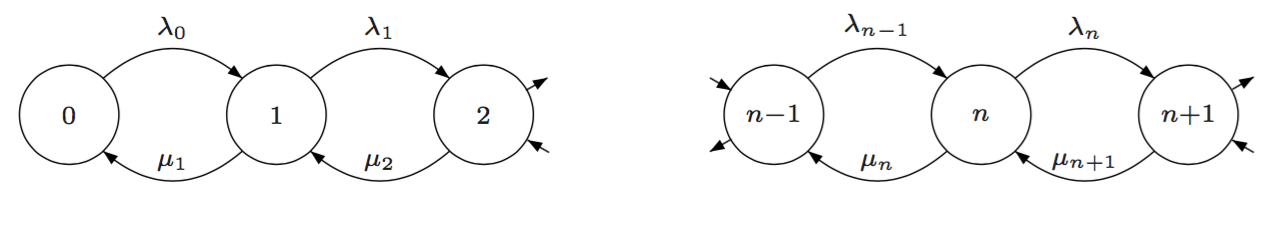
\includegraphics[width=0.9\textwidth]{img/grafo.png}
  \label{fig:ejemplo}
\end{figure}
\end{frame}
\section{Probabilidades de transición}
\begin{frame}
    \frametitle{Probabilidades de transición}
    Esto es una introducción
\end{frame}

\section{Ecuación de Kolmogorov}
\begin{frame}
    \frametitle{Ecuación de Kolmogorov}
    Esto es una introducción
\end{frame}

\section{Clasificación de los estados}
\begin{frame}
    \frametitle{Clasificación de los estados}
    Esto es una introducción
\end{frame}

\section{Teoremas límite}
\begin{frame}
    \frametitle{Teoremas límite}
    Esto es una introducción
\end{frame}

\section{Ejemplos}
\subsection{Ejemplo 1}
\begin{frame}
    \frametitle{Ejemplos}
    Esto es una introducción
\end{frame}
\begin{frame}
    \frametitle{Ejemplo 1}
    Esto es una introducción
\end{frame}
\end{document}
